
% Default to the notebook output style

    


% Inherit from the specified cell style.




    
\documentclass[11pt]{article}
\usepackage{fontspec}
\newfontfamily{\defaultfont}{Abhaya Libre}
\newfontfamily{\sinhalafont}{Abhaya Libre}
\usepackage[Sinhala, Latin]{ucharclasses}
\setDefaultTransitions{\defaultfont}{}
\setTransitionTo{Sinhala}{\sinhalafont}
\usepackage{amsmath} % AMS Math Package
\usepackage{amsthm} % Theorem Formatting
\usepackage{amssymb}	

    \begin{document}
    
    \title{ ඒ ලෙවල් ඉවරයි!}
    \maketitle
    
    

    
    හුදෙක් උසස් පෙළ නොස්ටැල්ජියානු මතකය ආවර්ජනය කිරීම උදෙසා....

උපුටා ගැනීම, වී. ජෝසප් හා කේ. පී. ඩී. ධර්මදාස විසින් සම්පාදිත
\emph{ගතිකය} කෘතියේ 3.35 අභ්‍යාසය.

\subsection{ගැටළුව}\label{uxd9cuxda7uxdc5uxdc0}

ප්‍රිස්මයක මධ්‍ය හරස්කඩ \(ABC\) ත්‍රිකෝණයකි.
\(A\hat{C}B=\frac{\pi}{2}\),
\(C\hat{A}B=\alpha \left(>\frac{\pi}{4}\right)\), \(AB=a\). ස්කන්ධය
\(M\) වන ප්‍රිස්මය \(AB\) සුමට තිරස් මේසයක් මත ස්පර්ෂ කරමින් නිසලව
පවතියි. එකක ස්කන්ධය \(m\) වන සමාන අංශු දෙකක් \(C\) ඉහළ ම ලක්ෂ්‍යයේ තබා,
ප්‍රිස්මයේ \(CA\), \(CB\) පාද ඔස්සේ පහළට ලිස්සා යාමට ඉඩ හරිනු ලැබේ.

\(\sqrt{\frac{2a\cot\alpha}{g}}\) කාලයක් ප්‍රිස්මය නිසලව පවතින බව ද, ඉන්
පසු

\(\frac{mg\sin\alpha\cos\alpha}{M+m\cos^2\left(\alpha\right)}\)
ත්වරණයෙන් චලනය වන බව ද පෙන්වන්න.

\subsection{නිර්බාධ වස්තු
සටහන}\label{uxdb1uxdbbuxdb6uxdb0-uxdc0uxdc3uxdad-uxdc3uxda7uxdc4uxdb1}

\begin{figure}
\centering
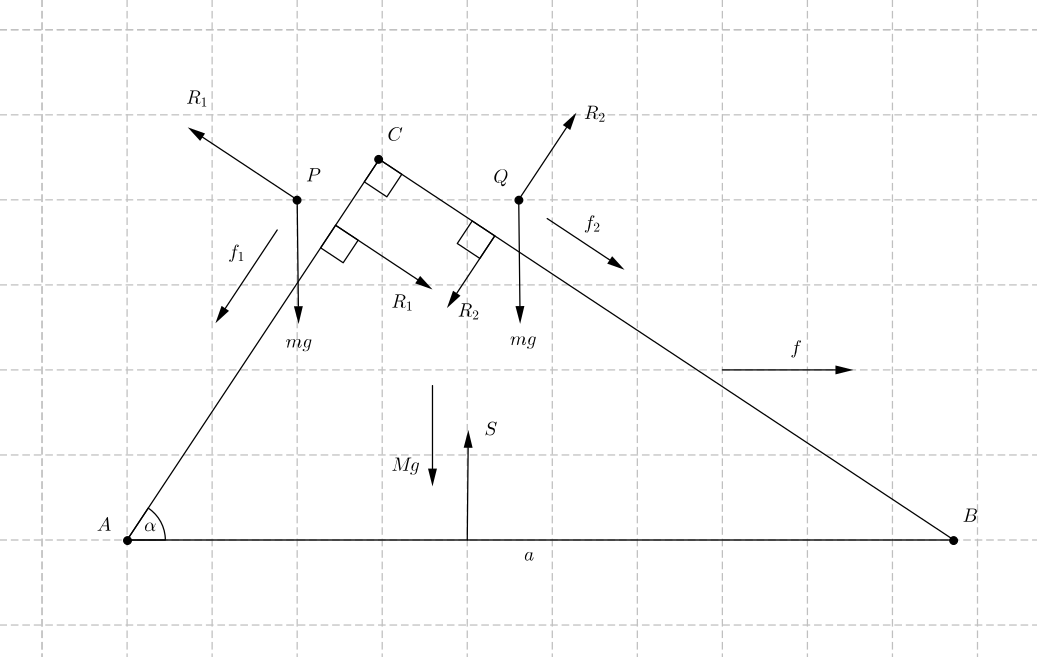
\includegraphics{free_body_diag.png}
\caption{}
\end{figure}

මෙහි \(f_1, f_2\) ත්වරණ ප්‍රිස්මයට සාපේක්ෂවත් \(f\) ත්වරණය පොළොවට
සාපේක්ෂවත් වේ.

\subsection{විසඳුම}\label{uxdc0uxdc3uxdb3uxdb8}

පද්ධතියට තිරසට \(F=ma\),

\[ 0 = Mf + m(f-f_1\cos\alpha) + m(f + f_2\sin\alpha)\tag{1} \]

\(P\) ට \(CA\) දෙසට \(F=ma\),

\[ mg\sin\alpha = m(f_1 - f\cos\alpha)\tag{2}\]

\(Q\) ට \(CB\) දෙසට \(F=ma\),

\[ mg\cos\alpha = m(f_2 + f\sin\alpha)\tag{3}\]

\((1), (2)\) හා \((3)\) මඟින් \(f=0\) බව පෙන්විය හැකිය.

අංශු දෙකම ප්‍රිස්මය හා ස්පර්ෂව පවතින තාක් \(f=0\) ව පවතියි.

\((2)\) න් \(f_1 = g\sin\alpha\), \(\therefore\) \(P\) හි පහළට ත්වරණය
\(f_1\sin\alpha=g\sin^2\alpha\)

\((3)\) න් \(f_2 = g\cos\alpha\), \(\therefore\) \(Q\) හි පහළට ත්වරණය
\(f_1\cos\alpha=g\cos^2\alpha\)

\(\alpha>\frac{\pi}{4}\) බැවින් \(\sin\alpha>\cos\alpha\)

මුලින් \(P\) ප්‍රිස්මය හැර යයි.

එයට ගත වන කාලය,

\(S=ut+\frac{1}{2}at^2\) සිරස්ව පහළට \(P\)ට යෙදීමෙන්,

\(a\cos\alpha\sin\alpha=0+\frac{1}{2}g\sin^2\left(\alpha\right) t^2\)

\(t = \sqrt{\frac{2a\cot\alpha}{g}}\)

\(P\) ඉවත් වූ පසුව \((1), (2)\) හා \((3)\) හි \(P\) ට අදාළ \(m\) පද
ශුන්‍ය කළ හැකිය.

එවිට \((1)\) සමීකරණය පහත ලෙස ශේෂ වේ:

\[0=Mf+m(f+f_2\sin\alpha)\tag{4}\]

\((3)\) හා \((4)\) විසඳීමෙන්,

\[f=-\frac{mg\sin\alpha\cos\alpha}{M+m\cos^2\left(\alpha\right)}\]

පිළිතුර ලද හැකිය.


    % Add a bibliography block to the postdoc
    
    
    
    \end{document}
